\documentclass{beamer}

\usepackage[italian]{babel}
\usepackage[T1]{fontenc}
\usepackage{beamerthemeAntibes}
\usepackage{graphicx}
\usepackage{listings}
\usepackage[utf8]{inputenc} 
\usepackage{epsfig}  
\usepackage{amsmath} 
\usepackage{multicol}
\usepackage{amsfonts}
\usepackage{hyperref}
\usepackage{listings}

\lstset{
  basicstyle=\footnotesize,
  language=C,                % choose the language of the code                 % where to put the line-numbers
  backgroundcolor=\color{white},  % choose the background color. You must add \usepackage{color}
  showspaces=false,               % show spaces adding particular underscores
  showstringspaces=false,         % underline spaces within strings
  showtabs=false,                 % show tabs within strings adding particular underscores
  tabsize=2,                      % sets default tabsize to 2 spaces
  captionpos=b,                   % sets the caption-position to bottom
  breaklines=true,                % sets automatic line breaking
  breakatwhitespace=true,         % sets if automatic breaks should only happen at whitespace
  title=\lstname,                 % show the filename of files included with \lstinputlisting;
}



\setbeamertemplate{itemize/enumerate body begin}{\footnotesize}

\title{Threshold-Free Cluster Enhancement}
\author{Luigi Giugliano$^1$, Marco Mecchia$^1$}
\institute{$^1$Università degli studi di Salerno}


\begin{document}

\begin{frame}
   \maketitle
\end{frame}

\begin{frame}
  \frametitle{Overview}
  \footnotesize \tableofcontents
\end{frame}

\AtBeginSection[]
  {
     \begin{frame}<beamer>
     \frametitle{Overview}
   \footnotesize \tableofcontents[currentsection]
     \end{frame}
}

\section{Introduzione al problema}

\subsection{Generazione delle mappe statistiche da FMRI}

\begin{frame}
\frametitle{Mappa statistica associata ad un esperimento FMRI}
\begin{block}{Mappa statistica}
Per un dato esperimento di \emph{Risonanza Magnetica Funzionale (FMRI)}, una \alert{mappa statistica} \'e un immagine in cui ad ogni voxel corrisponde un valore statistico.
\end{block}
\begin{itemize}
\item Solitamente, tali valori rappresentano la \emph{significativit\'a statistica} di attivazioni neuronali avvenute durante l'esperimento.
\item Le attivazioni vengono stimate attraverso il \alert{GLM}, su cui viene fatta \emph{inferenza} per ottenere i valori statistici.
\end{itemize}
\end{frame}
\begin{frame}{GLM - Aspetti teorici (1/3)}

Il \alert{Generelized Linear Model (GLM)} descrive il comportamento di ogni voxel con la seguente equazione:

$$Y = X\beta + \epsilon$$ 

\begin{block}{Genaralized Linear Model}
Descrive la risposta $y$ in termini della combinazione lineare di tutti i fattori in gioco ($X\beta$), includendo l'errore $\epsilon$.
\end{block}

\end{frame}

\begin{frame}
\frametitle{GLM - Aspetti teorici (2/3)}
Osservando l'intensit\'a dei voxel nel tempo, si ottiene il \alert{vettore delle osservazioni}.

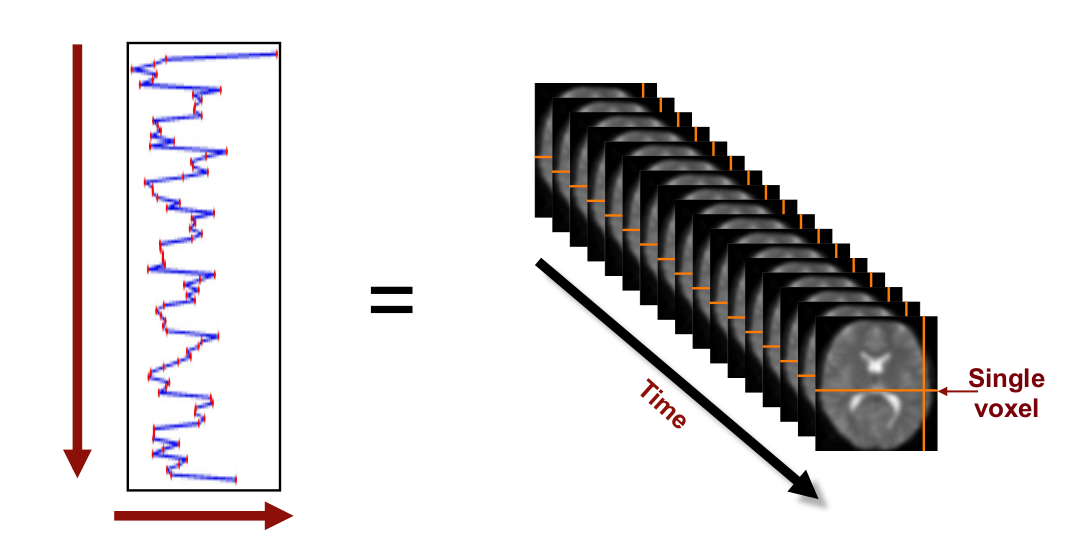
\includegraphics[keepaspectratio, width = 300px	]{Images/glm_matrix.png}
\end{frame}

\begin{frame}
\frametitle{GLM - Aspetti teorici (3/3)}
Come per i voxel, anche i predittori hanno una certa durata temporale.

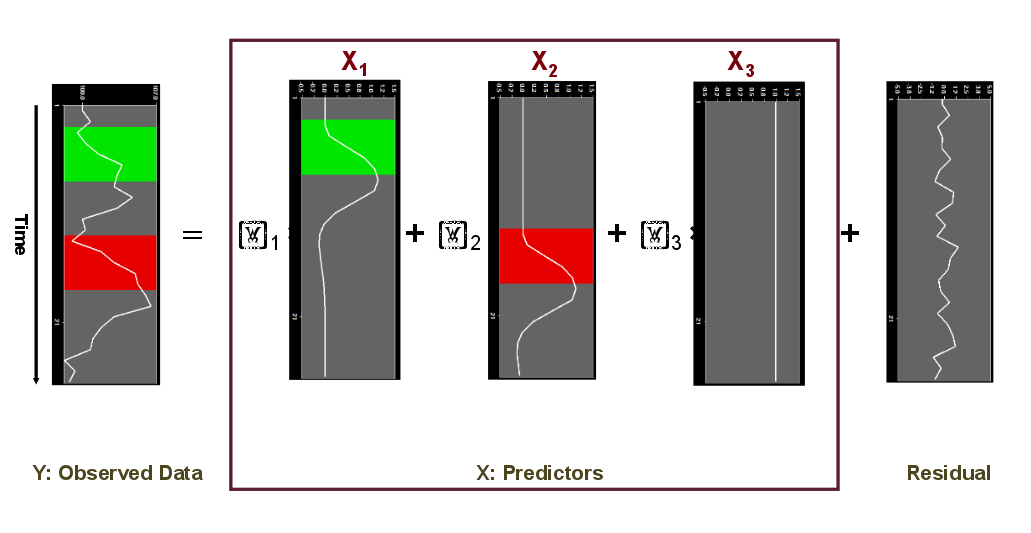
\includegraphics[keepaspectratio, width = 300px]{Images/glm_visual.png}
\end{frame}

\begin{frame}
\frametitle{GLM - Riepilogo}
Tenendo conto degli aspetti appena visti, il modello completo del GLM diventa:

$$Y = \beta X + \epsilon$$

dove:
\begin{itemize}
\item $Y$ \'e il vettore $N \times 1 $ dei dati osservati.
\item $X$ \'e la matrice $N \times r$ a rango pieno dei predittori.
\item $\beta$ \'e il vettore $r \times 1$ dei coefficienti di regressione.
\item $\epsilon$ \'e il vettore $N \times 1$ degli errori casuali.
\end{itemize}
\end{frame}

\begin{frame}
\frametitle{GLM - Stima dei $\beta$}
Il numero dei parametri spesso \'e $<<$ del numero di data point, per cui tra le infinite soluzioni del sistema si sceglie quella che minimizza l'errore residuale, cio\'e la \alert{stima dei minimi quadrati}:

$$ 	\hat{\beta} = (X^TX)^{-1} X^TY$$

Nei casi in cui $(X^TX)$ risulti non invertibile, si utilizza la \emph{Pseudoinversa di Monroe}.
\end{frame}

\begin{frame}
\frametitle{GLM - Inferenza statistica(1/2)}

\begin{itemize}
\item Per poter effettuare inferenza statistica sui valori restituiti dal GLM, occorre stimare la \alert{varianza del residuale}.
\item Si suppone che il rumore abbia una distribuzione \emph{gaussiana}, per cui \'e possibile stimare la varianza tramite la \emph{distribuzione chi quadrato}:
\end{itemize}
 
$$\hat{\sigma}^2 = \frac{\epsilon^T\epsilon}{J - p} \sim \sigma^2 \frac{\chi^2_{J-p}}{J-p}$$

dove: 
\begin{itemize}
\item $\epsilon$ \'e il rumore.
\item $J$ \'e il numero di data points.
\item $p = rank(X) $ \'e il numero di parametri indipendenti introdotto.
\item $J-p$ rappresenta il numero di \alert{gradi di libert\'a} del GLM.
\end{itemize}
\end{frame}

\begin{frame}
\frametitle{GLM - Inferenza statistica(2/2)}
Se la matrice $X$ \'e a rango pieno allora:
$$\hat{\beta} \sim \mathcal{N}(\beta, \sigma^2(X^TX)^{-1})$$
Segue che qualunque combinazione lineare dei $\beta$, cio\'e un \alert{contrasto statistico} segue la stessa distribuzione:
$$c^T\hat{\beta} \sim \mathcal{N}(c^T\beta, c^T\sigma^2(X^TX)^{-1}c)$$
Pertanto, dopo la stima, si calcola direttamente il parametro T:
$$T = \frac{c^T\hat{\beta} - d}{\sqrt{\hat{\sigma}^2c^T(X^TX)^{-1}c}}$$
\end{frame}


\subsection{Sogliatura delle immagini statistiche}
\begin{frame}
\frametitle{Sogliatura delle immagini statistiche}
\begin{block}{Sogliatura statistica}
Generalmente, in statistica \alert{la sogliatura} \'e un processo che permette di visualizzare i risultati di un esperimento maggiori di una soglia scelta. 
\end{block}

\bigskip

Una soglia ben scelta consente di visualizzare solo i risultati pi\'u significativi di un esperimento, eliminando in parte il rumore.
\end{frame}

\subsection{Sogliatura basata su cluster}
\begin{frame}
\frametitle{Spatial information enhancing}
Lo spatial information enhancing \'e una tecnica particolarmente utile per la sogliatura di mappe statistiche derivate da FMRI:
\smallskip
\begin{itemize}

\item le informazioni spaziali vengono usate per aumentare l'autenticità di estese aree di segnale. 
\medskip
\item le regioni del segnale sono infatti più estese del rumore e quindi trovare tali zone aumenta la possibilità che esse siano segnale e non artefatti.
\end{itemize}

\end{frame}

\begin{frame}
\frametitle{Cluster-based Thresholding}
Il cluster-based thresholding \'e l'approccio pi\'u comune in neuroimaging:
\smallskip
\begin{itemize}
\item Consiste nel visualizzare solo i voxel che fanno parte di aree la cui estensione \'e $\geq$ di una soglia fissata. 
\medskip
\end{itemize}
Problemi:
\begin{itemize}
\item Necessit\'a di definire una soglia di clustering.
\item Sogliatura di tipo \emph{hard}.
\item Difficolt\'a nel riconoscimento di eventuali \emph{subcluster}.
\end{itemize}
\end{frame}

\section{L'algoritmo TFCE}
\begin{frame}
\frametitle{TFCE}
TFCE tenta di superare i problemi degli approcci precedenti.
\begin{itemize}
\item Input: Una mappa statistica di qualsiasi tipo(T, Z, F).
\item Output: Una mappa statistica in cui il valore di ogni voxel \'e un \alert{punteggio} che rappresenta il contributo spaziale del cluster di cui fa parte.
\end{itemize}
\bigskip
\begin{itemize}
\item Clustering dell'immagine \alert{intrinseco}.
\end{itemize}
\end{frame}

\subsection{Calcolo dei punteggi}

\begin{frame}
\frametitle{Assegnazione dei punteggi (1/2)}
Il punteggio del voxel $p$ viene stabilito dalla seguente formula:

$$TFCE(p)=\int_{h=h_0}^{h_p}e(h)^E h^H dh$$
dove:
\begin{itemize}
\item $h_p$ \'e il \alert{valore statistico} del voxel $p$.
\item $e(h)$ \'e l'\alert{area del cluster} ad altezza $h$.
\item $E$ ed $H$ sono costanti.
\end{itemize}
\vfill
Questo integrale viene calcolato approssimandolo con una sommatoria ponendo $dh = 0.1$.

\end{frame}

\begin{frame}
\frametitle{Assegnazione dei punteggi (2/2)}
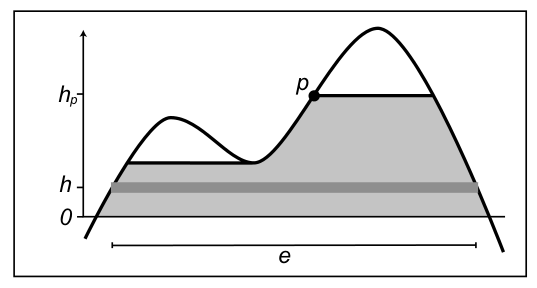
\includegraphics[width=300px]{Images/TFCE.png}
\end{frame}

\subsection{Calcolo dell'estensione dei cluster}

\begin{frame}
\frametitle{Calcolo estensione cluster (1/2)}
\begin{itemize}
\item Il calcolo dell'estensione del cluster nel caso di immagini tridimensionali risulta essere pi\'u complesso.
\item Occorre controllare il vicinato di ogni voxel in base alla \alert{26 connectivity}.
\end{itemize}
\center
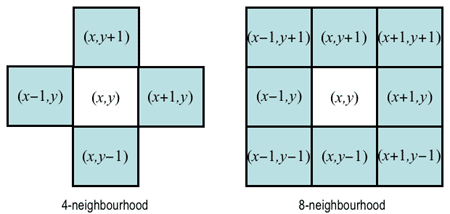
\includegraphics[width=250px]{Images/connectivity.png}
\end{frame}

\begin{frame}
\frametitle{Calcolo estensione cluster (2/2)}
La nostra implementazione consiste in un semplice algoritmo:
\begin{enumerate}
\item Viene generata, a partire dall'immagine statistica, una mappa binaria in base alla soglia $h$ corrente.
\item Una visita in ampiezza della mappa binaria etichetta tutti i cluster.
\end{enumerate}
\[
\begin{bmatrix}
    1       & 1 & 0 & 1 & 1\\
    1       & 1 & 0 & 0 & 0 \\
    1       & 0 & 0 & 1 & 1
\end{bmatrix}
\rightarrow
\begin{bmatrix}
    1       & 1 & 0 & 3 & 3\\
    1       & 1 & 0 & 0 & 0 \\
    1       & 0 & 0 & 2 & 2
\end{bmatrix}
\]
\begin{enumerate}
\setcounter{enumi}{2}
\item Per ogni voxel della mappa, il valore $e(h)$ \'e il numero di elementi presenti nel cluster di cui fa parte.
\end{enumerate}
\[
\begin{bmatrix}
    1       & 1 & 0 & 3 & 3\\
    1       & 1 & 0 & 0 & 0 \\
    1       & 0 & 0 & 2 & 2
\end{bmatrix}
\rightarrow
\begin{bmatrix}
    5       & 5 & 0 & 2 & 2 \\
    5       & 5 & 0 & 0 & 0 \\
    5       & 0 & 0 & 2 & 2
\end{bmatrix}
\]

\end{frame}

\subsection{Stima dei parametri}

\begin{frame}
\frametitle{Scelta dei parametri E ed H (1/2)}
Ricordando la formula di assegnazione dei punteggi:
$$TFCE(p)=\int_{h=h_0}^{h_p}e(h)^E h^H dh$$
\begin{itemize}
\item La scelta dei parametri $E$ ed $H$ risulta essere cruciale per avere dei punteggi coerenti.

\item Tali parametri sono stati scelti in modo da adattarsi ad un ampio set di segnali e rumore.

\end{itemize}
\end{frame}

\begin{frame}
\frametitle{Scelta dei parametri E ed H (2/2)}
La scelta finale \'e stata $H = 2$ ed $E = 0.5$ poich\'e:
\bigskip
\begin{itemize}

\item Scegliere $H > 1$ ha il risultato di far si che gli score scalino pi\'u che linearmente con l' ``altezza'' dei cluster.
\begin{itemize}
\item Ci\'o \'e desirabile in quanto vengono favoriti cluster di intensit\'a molto alta rispetto a quelli con intensit\'a pi\'u bassa.
\end{itemize}
\medskip
\item Scegliere $E < 1$ fa si che il risultati scali meno che linearmente con la ``larghezza'' dei cluster.
\begin{itemize}
\item Ci\'o \'e desirabile specie con $h$ molto basso poich\'e \'e probabile che ci siano pochi cluster di dimensioni molto grandi, che forniscono poca informazione spaziale.
\end{itemize}


\end{itemize}
\end{frame}

\subsection{Test delle permutazioni}
\begin{frame}
\frametitle{Sogliatura esplicita}
\begin{itemize}
\item \onslide<1->L'algoritmo TFCE produce un'immagine con gli score calcolati sull'immagine originale.

\item \onslide<2->Tuttavia, l'immagine prodotta manca di \emph{valenza statistica}.

\item \onslide<3->Per calcolare la valenza statistica dell'immagine degli score, occorre calcolare i \alert{p-value} per ogni voxel.

\item \onslide<4->Essendo TFCE una particolare statistica che sfrutta informazioni spaziali, \'e possibile calcolare i p-value effettuando il \alert{test delle permutazioni} sull'esperimento originale.
\end{itemize}
\end{frame}

\begin{frame}
\frametitle{Test delle permutazioni applicato al GLM single study(1/2)}
\begin{itemize}
\item \onslide<1-> Il GLM asserisce che il comportamento di ogni voxel pu\'o essere descritto dalla legge $Y = \beta X + \epsilon$.
\item \onslide<2->Sotto l'ipotesi nulla $\mathcal{H}_0 : \beta = 0 \implies Y = \epsilon$, cio\'e i dati sono puro rumore.
\item \onslide<3->Sotto questa ipotesi, i voxel osservati $Y$ possono essere quindi \alert{permutati}.
\item \onslide<4-> In caso di assenza di variabili di disturbo, permutare i predittori e' equivalente:
\end{itemize}
$$PY = X\beta + \epsilon \iff Y = P'X\beta + P'\epsilon$$
\end{frame}

\begin{frame}
\frametitle{Test delle permutazioni applicato al GLM single study(2/2)}
\begin{itemize}
\item \onslide<1->Data la \emph{permutabilit\'a} garantita dall'ipotesi nulla, i dati osservati possono derivare in maniera equiprobabile da qualsiasi condizione sperimentale.
\item \onslide<2->Ci\'o vale anche per la statistica calcolata a partire dai dati.
\item \onslide<3->La \alert{distribuzione delle permutazioni} \'e quindi l'insieme delle statistiche calcolate dalle possibili permutazioni dei dati di partenza.
\item \onslide<4->Tale distribuzione ci consente di formalizzare la probabilit\'a di un certo risultato.
\end{itemize}
\begin{block}{P-value}
Il P-value \'e la proporzione dei valori statistici nella distribuzione delle permutazioni che sono maggiori o uguali del valore osservato nell'esperimento.
\end{block}
\end{frame}

\begin{frame}
\frametitle{Test delle permutazioni - Casi particolari}
Il semplice modello appena visto pu\'o essere esteso a diversi casi:
\begin{itemize}
\item Il modello di Freedman-Lane tiene conto di variabili di disturbo, ed \'e quello utilizzato dall'algoritmo \emph{Randomise}
\item Negli studi di gruppo, il caso \'e ancora pi\'u semplice: i blocchi di permutazione sono definiti dai pazienti.
\end{itemize}
Per ulteriori approfondimenti consultare:

\center\href{http://www.sciencedirect.com/science/article/pii/S1053811914000913}{Permutation inference for the general linear model}
\end{frame}

\section{Confronto risultati}
\subsection{Montecarlo simulation - BrainVoyager}
\begin{frame}
\frametitle{Metodo di montecarlo per la sogliatura basata su cluster}
Il metodo prende in input una soglia di significatività $\alpha$ e restituisce la taglia del cluster a cui sogliare.
\begin{itemize}
\item Vengono generate $n$ mappe statistiche random con il metodo di Montecarlo
\item Od ogni mappa viene applicato uno smoothing spaziale calcolato sulla mappa di input
\item Si sceglie la taglia $t$ tale che la probabilità di osservare cluster generati casualmente di taglia maggiore di $t$ sia uguale ad $\alpha$
\end{itemize}
Il valore così ottenuto viene utilizzato per la sogliatura basata su cluster. 
\end{frame}

\subsection{Altri metodi di correzione - BrainVoyager}
\begin{frame}
\frametitle{Bonferroni}
In statistica la \textbf{correzione di Bonferroni} viene utilizzata per contrastare il problema dei confronti multipli.\\
\medskip
E' basata sull'idea che se in un esperimento si stanno testando $m$ ipotesi, un modo per mantenere il \textbf{familywise error rate} (\textbf{FWER} = probabilità di effettuare errore di \textit{Tipo 1} all'inverno delle ipotesi) è quello di testare ogni ipotesi individualmente con una significanza statistica di $1/m$ moltiplicato per il livello massimo desiderato.\\
\medskip
Quindi se vogliamo un \textit{p-value} totale di $\alpha$, la correzione di Bonferroni testerà ogni singolo esperimento con un \textit{p-value} di $\alpha/m$ è rifiuterà l'ipotesi nulla se il \textit{p-value} di quell'esperimento è minore di tale valore.
\end{frame}

\begin{frame}
\frametitle{False Discovery Rate}
Il \textbf{False Discovery Rate} come la correzione di Bonferroni si prefigge l'obiettivo di contrastare il problema dei confronti multipli.\\
\smallskip
La procedura per il controllo FDR è stata creata per gestire la proporzione attesa di rifiuto dell'ipotesi nulla,  che però sarebbe stato sbagliato rifiutare ("false discoveries").\\
\smallskip
La procedura FDR fornisce un controllo meno stringente sugli errori di \textit{Tipo 1} rispetto a Bonferroni.
\end{frame}

\begin{frame}
Sia:
\begin{itemize}
\item $V$ il numero di falsi positivi (Errori di Tipo 1)
\item $S$ il numero di veri positivi 
\item $R =  V+S$ 
\end{itemize}
La FDR è definita:
\begin{equation*}
FDR = E\Big[\frac{V}{S+V}\Big] = E\Big[\frac{V}{S+V}\Big]
\end{equation*}
dove $\frac{V}{R} = 0$ quando $R = 0$.
\end{frame}

\begin{frame}
\framesubtitle{Procedura di controllo di Benjamini–Hochberg}
Avendo $H_1 \dots H_m$ test sull'ipotesi nulla e $p_1 \dots p_m$ \textit{p-value} corrispondenti. Ordiniamo i \textit{p-value} in ordine crescente; il \textit{p-value} più piccolo corrisponde al test con valore statistico più alto.\\
\smallskip
La procedura Benjamini–Hochberg controlla il false discovery rate (al livello $\alpha$) con i seguenti passi:\\
\medskip
\begin{enumerate}
\item Per un dato $\alpha$, trova il più grande $k$ per cui: $p_k \leq \frac{k}{m}\alpha$
\item Rifiuta l'ipotesi nulla (accetta come discovery vere) tutte i test $H_i \dot H_k$
\end{enumerate}
La procedura di Benjamini–Hochberg è valida quando i $m$ test sono indipendenti e soddisfa anche la seguente equazione:
\begin{equation*}
FDR \leq \frac{m_0}{m}\alpha \leq \alpha
\end{equation*}
\end{frame}


\subsection{TFCE - FSL}
\begin{frame}
\end{frame}

\subsection{TFCE - Brainvoyager}
\begin{frame}
\end{frame}

\section{Codice}
\subsection{Suddivisione del codice}
\begin{frame}
\frametitle{Suddivisione del codice}
I file principali che compongono il plugin sono:
\begin{itemize}
\item{Tfce.cpp}
\item{Utilities.cpp}
\end{itemize}
\vfill
\textbf{Tfce} è il core del plugin, dove avviene il calcolo dei punteggi.\\
\smallskip
\textbf{Utilities} contiene tutte le funzioni di supporto.
\end{frame}

\begin{frame}[fragile]
\frametitle{Funzioni pubbliche (1/3)}
L'unica funzione che viene esposta dal file \textbf{Tfce.h} è:
\begin{center}
\begin{lstlisting}
float * tfce_score(float * map, int dim_x, int dim_y, int dim_z, float E, float H, float dh);
\end{lstlisting}
\end{center}
\end{frame}

\begin{frame}[fragile]
\frametitle{Funzioni pubbliche (2/3)}
Le funzioni che espone \textbf{Utilities.h} sono:
\begin{center}
\begin{lstlisting}
void findMinMax(float *map, int n, float *min, float *max, float * range);

int * getBinaryVector(float * map, int n, int (*confront)(float, float), float value, int *      numOfElementsMatching);
\end{lstlisting}
\end{center}
\end{frame}

\begin{frame}[fragile]
\frametitle{Funzioni pubbliche (3/3)}
\begin{center}
\begin{lstlisting}
float * fromBinaryToRealVector(float * map, int n, int * binaryVector);

float * fill0(int n);

void apply_function(float * vector, int n, float (* operation) (float a, float b), float argument);

int linearIndexFromCoordinate(int x, int y, int z, int max_x, int max_y);

void coordinatesFromLinearIndex(int index, int max_x, int max_y, int * x, int * y, int * z);

float * copyAndConvertIntVector(int * vector, int n);
\end{lstlisting}
\end{center}
\end{frame}

\subsection{Dettagli implementativi}
\begin{frame}[fragile]
\frametitle{Funzione tfce score}
\begin{center}
\begin{lstlisting}
float * tfce_score(float * map, int dim_x, int dim_y, int dim_z, float E, float H, float dh){
	findMinMax(map, n, &minData, &maxData, &rangeData);
	precision = rangeData/dh;
	if (precision > 200) {
		increment = rangeData/200;
	} else{
		increment = rangeData/precision;	
	}
	steps = ceil((maxData - minData) / (increment));
	#pragma omp parallel for
	for (i = 0; i < steps; i++) {
		 computeTfceIteration(minData + i*increment, map, n, dim_x, dim_y, dim_z, E, H, dh, toReturn);
	}	
	return toReturn;
}
\end{lstlisting}
\end{center}
\end{frame}

\begin{frame}[fragile]
\frametitle{Funzione computeTfceIteration (1/3)}
\begin{center}
\begin{lstlisting}
void computeTfceIteration(float h, float * map, int n, int dim_x, int dim_y, int dim_z, float E, float H, float dh, float * toReturn){
	int * indexMatchingData = getBinaryVector(map, n, moreThan, h, &numOfElementsMatching);
	clustered_map = find_clusters_3D(indexMatchingData, dim_x, dim_y, dim_z, n, &num_clusters);
	extent_map = new int[n];
	for (j = 0; j < n; ++j){
		extent_map[j] = 0;
	}
	delete [] indexMatchingData;
\end{lstlisting}
\end{center}
\end{frame}

\begin{frame}[fragile]
\frametitle{Funzione computeTfceIteration (2/3)}
\begin{center}
\begin{lstlisting}

for (i = 1; i <= num_clusters; ++i) {
		numOfElementsMatching = 0;	
		for (j = 0; j < n; ++j){
		    if(clustered_map[j] == i)
		        numOfElementsMatching++; 
		}
		for (j = 0; j < n; ++j) {
		   if(clustered_map[j] == i)
		       extent_map[j] = numOfElementsMatching; 
		}
}
		      
\end{lstlisting}
\end{center}
\end{frame}

\begin{frame}[fragile]
\frametitle{Funzione computeTfceIteration (3/3)}
\begin{center}
\begin{lstlisting}
clustered_map_float = copyAndConvertIntVector(extent_map, n);
apply_function(clustered_map_float, n, elevate, E);
apply_function(clustered_map_float, n, multiply, pow(h, H));
apply_function(clustered_map_float, n, multiply, dh);
for (i = 0; i < n; ++i) {
#pragma omp atomic
    toReturn[i] += (clustered_map_float[i]);
}
delete[] clustered_map_float;
delete[] clustered_map;
delete[] extent_map;
\end{lstlisting}
\end{center}
\end{frame}

\begin{frame}[fragile]
\frametitle{Funzione getBinaryVector}
Questa funzione emula il risultato del costrutto Matlab (matrice <condizione> valore).
\begin{center}
\begin{lstlisting}
int * getBinaryVector(float * map, int n, int (*confront)(float, float), float value, int * numOfElementsMatching){
    int * binaryVector = new int [n];
    (*numOfElementsMatching) = 0;
    int i;
    for (i = 0; i < n; ++i) {
        if(confront(map[i],value)){
            binaryVector[i] = 1;
            (*numOfElementsMatching)++;
        }
        else
            binaryVector[i] = 0;
    }
    return binaryVector;
}
\end{lstlisting}
\end{center}
\end{frame}

\begin{frame}[fragile]
\frametitle{Calcolo dell'estensione dei cluster}
La funzione \textbf{find\_cluster\_3D}:\\
\begin{lstlisting}
int * find_clusters_3D(int * binaryVector, int dim_x, int dim_y, int dim_z, int n, int * num_clusters)
\end{lstlisting}

restituisce la mappa dei cluster trovati utilizzando la \textbf{26-connectivity} nell'immagine binaria fornita in input.
\end{frame}

\begin{frame}[fragile]
E' stato utilizzata la specifica OpenMP per rendere il calcolo degli score più veloce.\\
\medskip
OpenMP (Open Multiprocessing) è un API multipiattaforma per la creazione di applicazioni parallele su sistemi a memoria condivisa.\\
\smallskip
Il comando:\\
\textbf{\#pragma omp parallel for}\\
viene utilizzato per rendere un for parallelo.\\
\smallskip
Il comando:\\
\textbf{\#pragma omp atomic}\\
invece viene utilizzato per rendere un istruzione atomica.\\
\end{frame}

\begin{frame}
Abbiamo deciso di utilizzare, OMP perch\'e l'effort per utilizzarlo \'e praticamente nullo, e le prestazioni sono ottime.\\
\medskip
Inoltre essendo che l'implementazione dei \textit{Thread} in \textit{C} cambia tra Windows e Linux, si sarebbe reso necessario modificare il codice per renderlo funzionante su entrambe le piattaforme.
\end{frame}

\section{Conclusioni}
\begin{frame}
\end{frame}


\end{document}
